\documentclass[]{beamer} 
\usetheme{Copenhagen}
\usecolortheme{default}

%\usepackage[ngerman]{babel}
\usepackage[latin1]{inputenc}
\usepackage{graphicx}
\usepackage{amsmath}
\usepackage{subfigure}
\usepackage{hyperref}

\input{jkcommands.tex}
\title{$B_{s}\rightarrow D_{s}K\pi\pi$ : BR measurement and $\gamma$ determination}
\author{Philippe d'Argent \inst{1}, Evelina Gersabeck \inst{1}, Matthieu Kecke \inst{1}, Manuel Schiller \inst{2}}
\institute{\inst{1} PI Heidelberg, \inst{2} CERN}
\date{25.01.2016}
\setbeamertemplate{footline}[page number]
\begin{document}
\frame{\titlepage}

\begin{frame}
\frametitle{Theory}

\begin{figure}
\includegraphics[width=9.5cm,height=6.0cm]{pics/CKMvincoli}
\end{figure}

$\gamma \equiv arg[-(V_{ud}V_{ub}^{*})/(V_{cd}V_{cb}^{*})]$ \newline

$\gamma$ can be studied using the interference between $b\rightarrow u$ and $b \rightarrow c$ transitions at tree level

\end{frame}

\begin{frame}
\frametitle{Why bother?}

$\gamma$ is the least well measured phase of the CKM triangle. Following results are obtained by averaging over several decay modes:

\begin{columns}

\column{.55\textwidth}
\begin{itemize}

\item LHCb: $\gamma = 73^{+9}_{-10}$

\item BaBar: $\gamma = 73^{+17}_{-16}$

\item Belle:  $\gamma = 68^{+15}_{-14}$

\end{itemize}


\column{.55\textwidth}
\begin{figure}
\includegraphics[width=6.0cm,height=4.0cm]{pics/summer14_gammaOUT_fullfit_gamma}
\end{figure}

\end{columns}

Precision of global fit $\approx 7\%$  v.s. the theory uncertainty of $<<1\%$  \newline \newline

$\rightarrow$ many unexplored channels left to improve the overall precision!

\end{frame}

\begin{frame}
\frametitle{And why this channel?}

\begin{figure}
\includegraphics[width=11.0cm,height=4.5cm]{pics/FeynmannGraphs}
\end{figure}

interference between a) and b) with same final state via mixing \newline

complimentary to $\gamma$ determination in $B_{s}\rightarrow D_{s}K$ \newline

technically interesting application of time dependent amplitude analysis 

\end{frame}


\begin{frame}
\frametitle{What has been done}

First observation and BR mesurement done with 1 $fb^{-1}$ and $N_{D_{s}K\pi\pi} = 216 \pm 22$ in 2012 (LHCb-ANA-2012-076): 

\[\frac{\mathcal{B}(B_{s}\rightarrow D_{s}K\pi\pi)}{\mathcal{B}(B_{s}\rightarrow D_{s}\pi\pi\pi)} = (5.2\pm 0.5 \pm 0.3) \cdot 10^{-2}\]
 

\begin{figure}
\includegraphics[width=5.5cm,height=3.7cm]{pics/BsDspipipi}
\subfigure{\includegraphics[width=5.5cm,height=3.7cm]{pics/BsDsKpipi}}
\caption{left: $D_{s}\pi\pi\pi$, right: $D_{s}K\pi\pi$}
\end{figure}


\end{frame}


\begin{frame}
\frametitle{Our plan}

We like to:
\begin{itemize}

\item redo the BR measurement with $3 fb^{-1}$ using $B_{s}\rightarrow D_{s}\pi\pi\pi$ as normalization channel

\item do a full time dependent daliz plot analysis to get strong phase difference and amplitude ratio across phase space to measure $\gamma$


\end{itemize} 

\bigskip

The analysis follows principle of $\gamma$ measurement in $B_{s}\rightarrow D_{s}K$, but with additional pion pair the dalitz analysis is necessary

\end{frame}


\begin{frame}
\frametitle{Stripping}

We produced Data and MC ntuples for 2011 and 2012:

\begin{tabular}{l|l|l}
Year & Channel & Stripping \\ \hline
2011 & $D_{s}K\pi\pi$ & B02DKPiPiD2HHHPIDBeauty2Charm, S21 \\
2012 & $D_{s}K\pi\pi$ & B02DKPiPiD2HHHPIDBeauty2Charm, S21\\
2011 & $D_{s}\pi\pi\pi$ & B02DPiPiPiD2HHHPIDBeauty2Charm, S21 \\
2012 & $D_{s}\pi\pi\pi$ & B02DPiPiPiD2HHHPIDBeauty2Charm, S21\\
\end{tabular} \newline

Additionally, we produced $B_{s}\rightarrow D_{s}^{*}X$ MC samples to constrain peaking background (see later) \newline

The plan is to use all possible final states, with $D_{s}\rightarrow KK\pi,K\pi\pi,\pi\pi\pi$ \newline

We expect O(1k) signal events

\end{frame}


\begin{frame}
\frametitle{Stripping Selection}
Stripping and (pre-)selection cuts include:

\begin{itemize}

\item all tracks: $p > 1$ $GeV$ , $p_{t} > 100$ $MeV$, $track\chi^{2}/ndof < 3$ and $IP\chi^{2} > 4$ 

\item $D_{s}$ daughter: $\Sigma p_{t} > 1.8$ $GeV$, max DOCA 0.5mm and $M_{KK\pi}$ within 100 $MeV$ of $M_{D_{s}}$  

\item $D_{s}$: $Vertex\chi^{2}/ndof < 10$ and min $FD\chi^{2} > 36$ 

\item $B_{s}$: $DIRA > 0.99$, min $IP\chi^{2} > 20$, $FD\chi^{2} > 100$ and vertex fit $\chi^{2}/ndof < 8$

\item loose PID requirements on the final state \\ kaons ($\Delta LL(K - \pi) > -5$) and pions ($\Delta LL(K - \pi) < 10$)

\end{itemize}

\end{frame}

\begin{frame}

\frametitle{Physical Background}

In addition to the previous cuts, we veto some specific backgrounds such as:

\begin{itemize}

\item $B_{s}\rightarrow D_{s}D_{s}$: \newline
 $|M(K\pi\pi) - m_{D_{s}}| > 20$ $MeV$

\item $B^{0}\rightarrow D^{+}(\rightarrow K\pi\pi)K\pi\pi$: \newline
 possible with single miss-ID. Vetoed by changing $K^{+}\rightarrow\pi^{+}$ mass hypothesis and check $|M(K^{+}\pi^{-}\pi^{+}) - m_{D^{+}}| > 20$ $MeV$ \newline
$||$ $\Delta LL(K - \pi) > 10$ for the $K^{+}$

\item $\Lambda_{b}^{0}\rightarrow \Lambda_{c}^{+}(\rightarrow Kp\pi)K\pi\pi$: \newline
 possible with single miss-ID. Vetoed by assigning $K^{+}\rightarrow p$ and check $|M(pK^{-}\pi^{+}) - m_{\Lambda_{c}^{+}}| > 15$ $MeV$ \newline
$||$ $\Delta LL(K - p) > 0$ for the $K^{+}$

\end{itemize}

\end{frame}

%
%\begin{frame}
%\frametitle{First plots}
%
%After the preselection of candidates we get (only $D_{s}\rightarrow KK\pi$):
%
 %\begin{figure}
%\includegraphics[width=5.5cm,height=3.7cm]{pics/mass_Bs_preSel_12Data_3pi.png}
%\subfigure{\includegraphics[width=5.5cm,height=3.7cm]{pics/mass_Bs_preSel_12Data.png}}
%\caption{invariant mass of left: $B_{s}\rightarrow D_{s}\pi\pi\pi$ candidates , right: $B_{s}\rightarrow D_{s}K\pi\pi$ candidates}
%\end{figure}
%
%
%$\rightarrow$ further selection via multivariate method
%
%\end{frame}


\begin{frame}
\frametitle{TMVA}

We take the upper mass sideband of $B_{s}$ data candidates as background and MC signal events \newline

Variables used for BDTG training, with $X_{s} = (K\pi\pi)$:

\begin{itemize}

\item $log(min(IP\chi^{2}))$ and $log(max(IP\chi^{2}))$ of $D_{s}$ daughters

\item $log(min(IP\chi^{2}))$ and $log(max(IP\chi^{2}))$ of $X_{s}$ daughters

\item $log((IP\chi^{2}))$ of $X_{s}$

\item $log((IP\chi^{2}))$ of $B_{s}$

\item FD significance of $B_{s}$ and $D_{s}$

\item $log(min(p_{t}))$ of $D_{s}$ and $X_{s}$ daughters

\item $B_{s}$ vertex fit $\chi^{2}$ 

\item $max(track\chi^{2})$

\item Cone $p_{t}$ asymmetry of all tracks 

\item max(track-ghostProb)

\end{itemize}

\end{frame}



\begin{frame}
\frametitle{BDTG output}

\begin{figure}
\includegraphics[width=5.5cm,height=4.0cm]{pics/BDT_Response_BDTG}
\subfigure{\includegraphics[width=5.5cm,height=4.0cm]{pics/BDT_Effizienz_BDTG}}
\caption{left: BDTG response, right: BDTG efficiency curves}
\end{figure}

We optimize our response cut using a massfit in the $B_{s}\rightarrow D_{s}\pi\pi\pi$ channel after pre-selection and scale the obtained value for S with the PDG BR and relative efficiency to $B_{s}\rightarrow D_{s}K\pi\pi$   


\end{frame}

\begin{frame}
\frametitle{Background Shape for normalization channel}

 %Physical background shape for $B_{s}\rightarrow D_{s}\pi\pi\pi$ (from MC):

 \begin{figure}
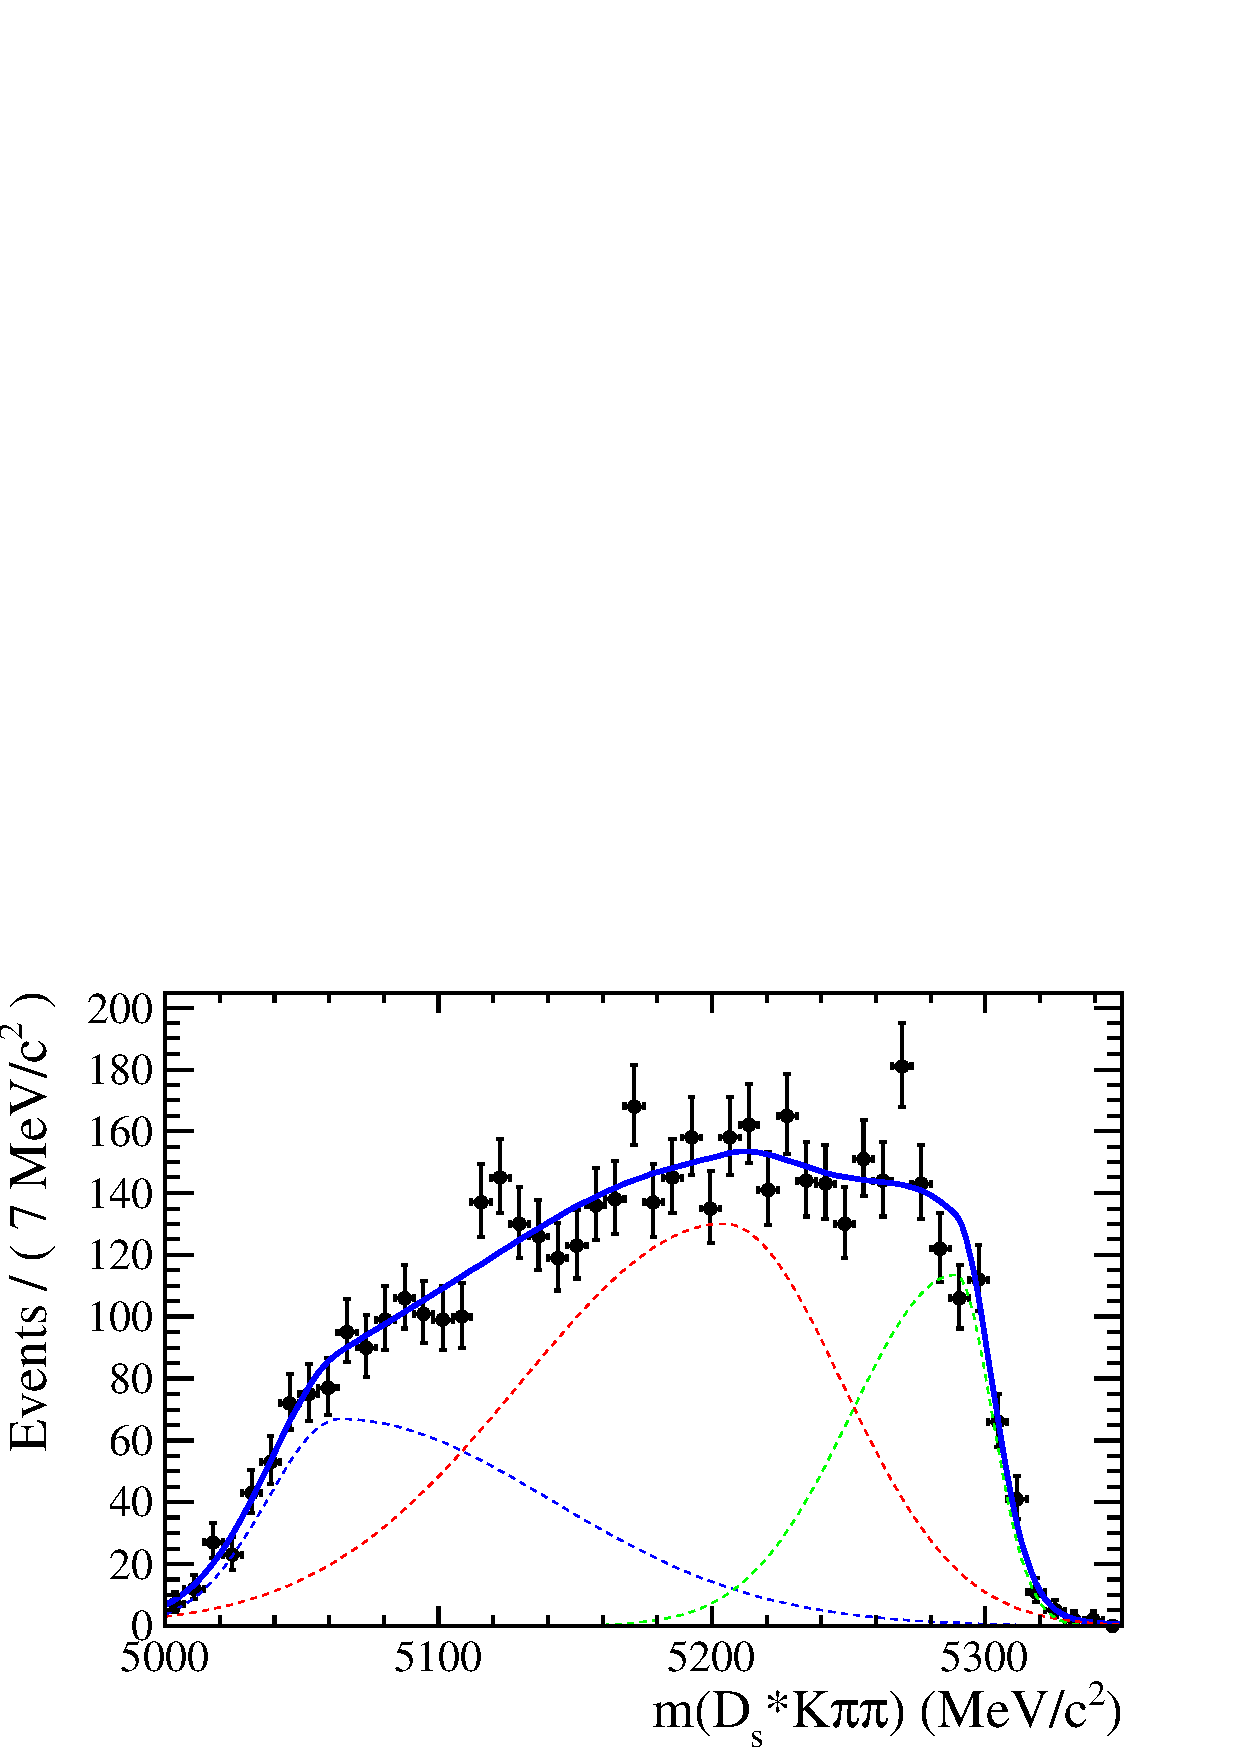
\includegraphics[width=8.0cm,height=5.5cm]{pics/Bs2Dsstartpipipi.png}
\caption{partially reconstructed $B_{s}\rightarrow D_{s}^{*}\pi\pi\pi$}
\end{figure}

\end{frame}

\begin{frame}
\frametitle{Background Shapes for signal channel}

 %Physical background shapes for $B_{s}\rightarrow D_{s}K\pi\pi$ (from MC):

\begin{figure}
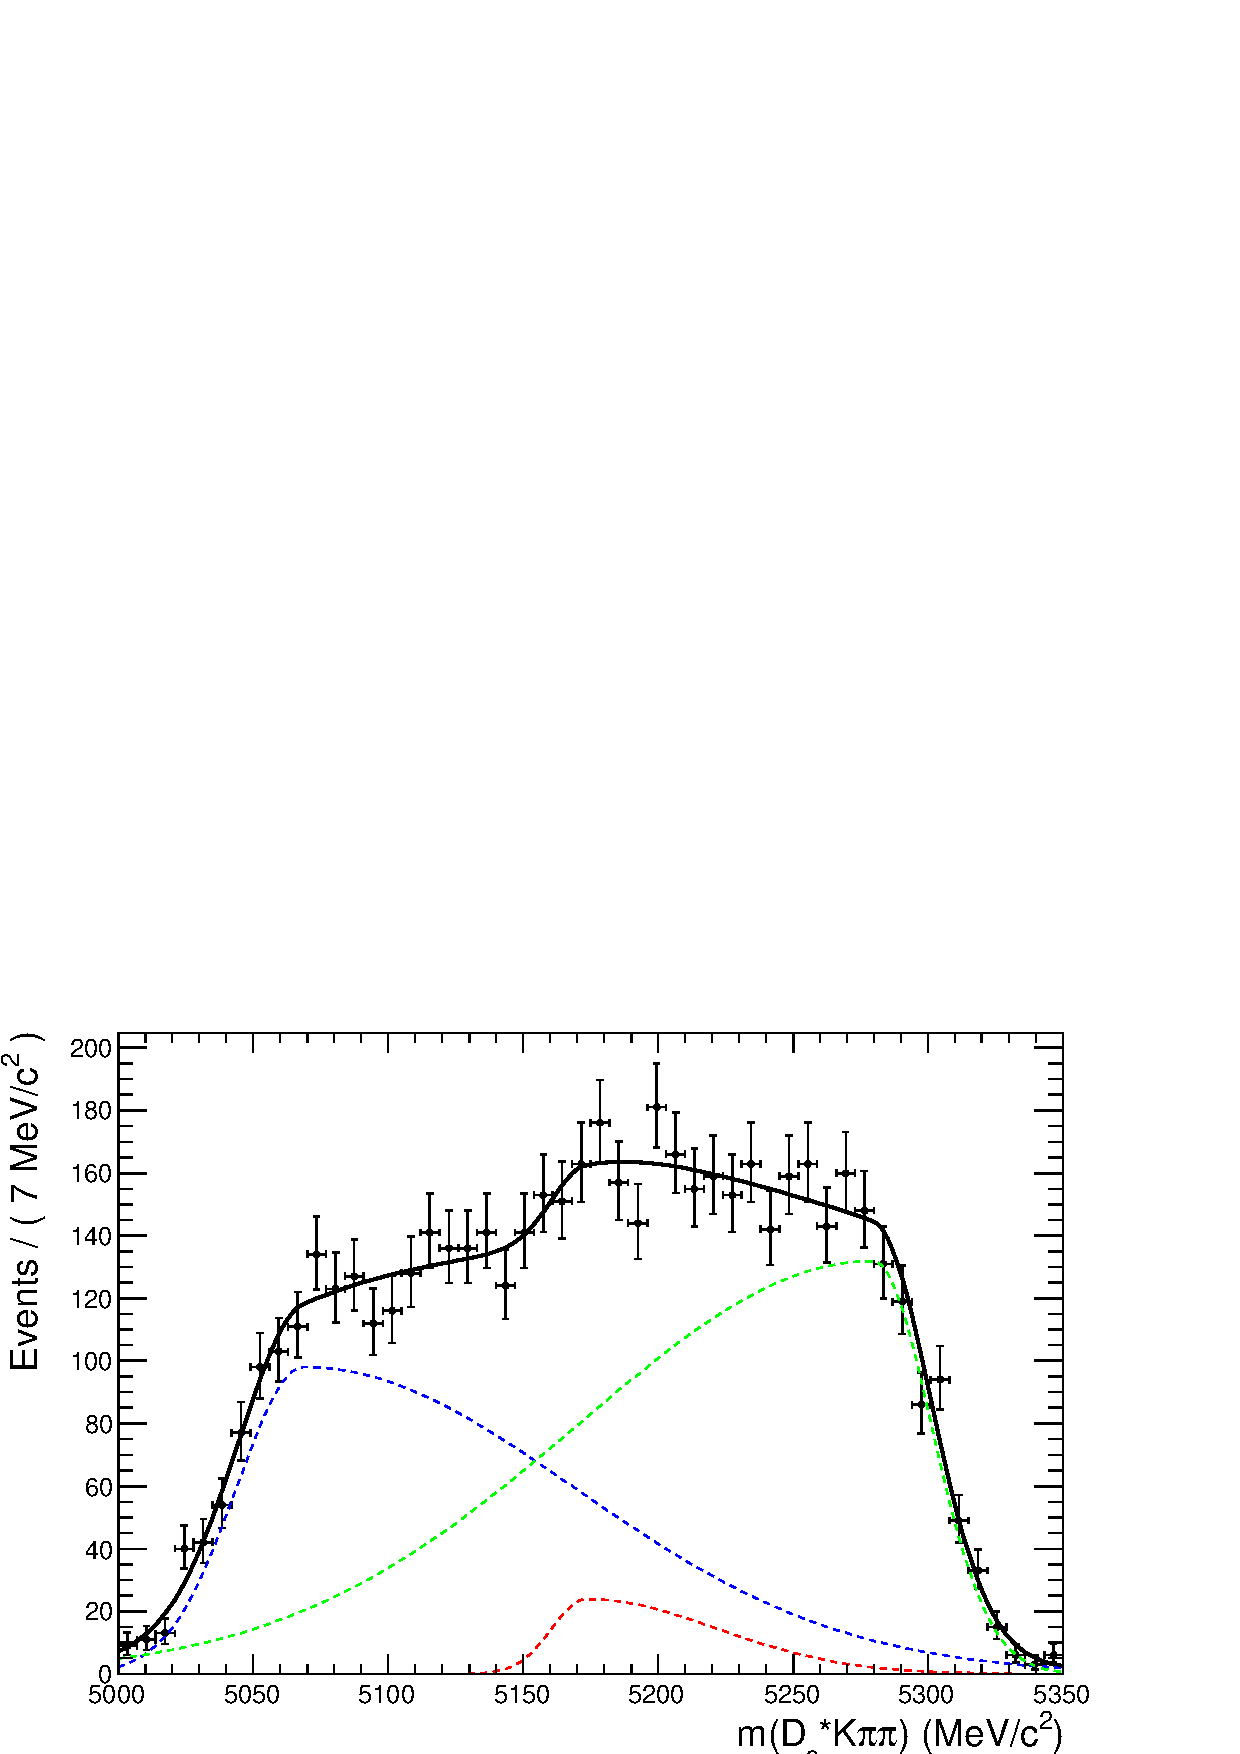
\includegraphics[width=4.5cm,height=2.0cm]{pics/Bs2DsstartKpipi.png}
\subfigure{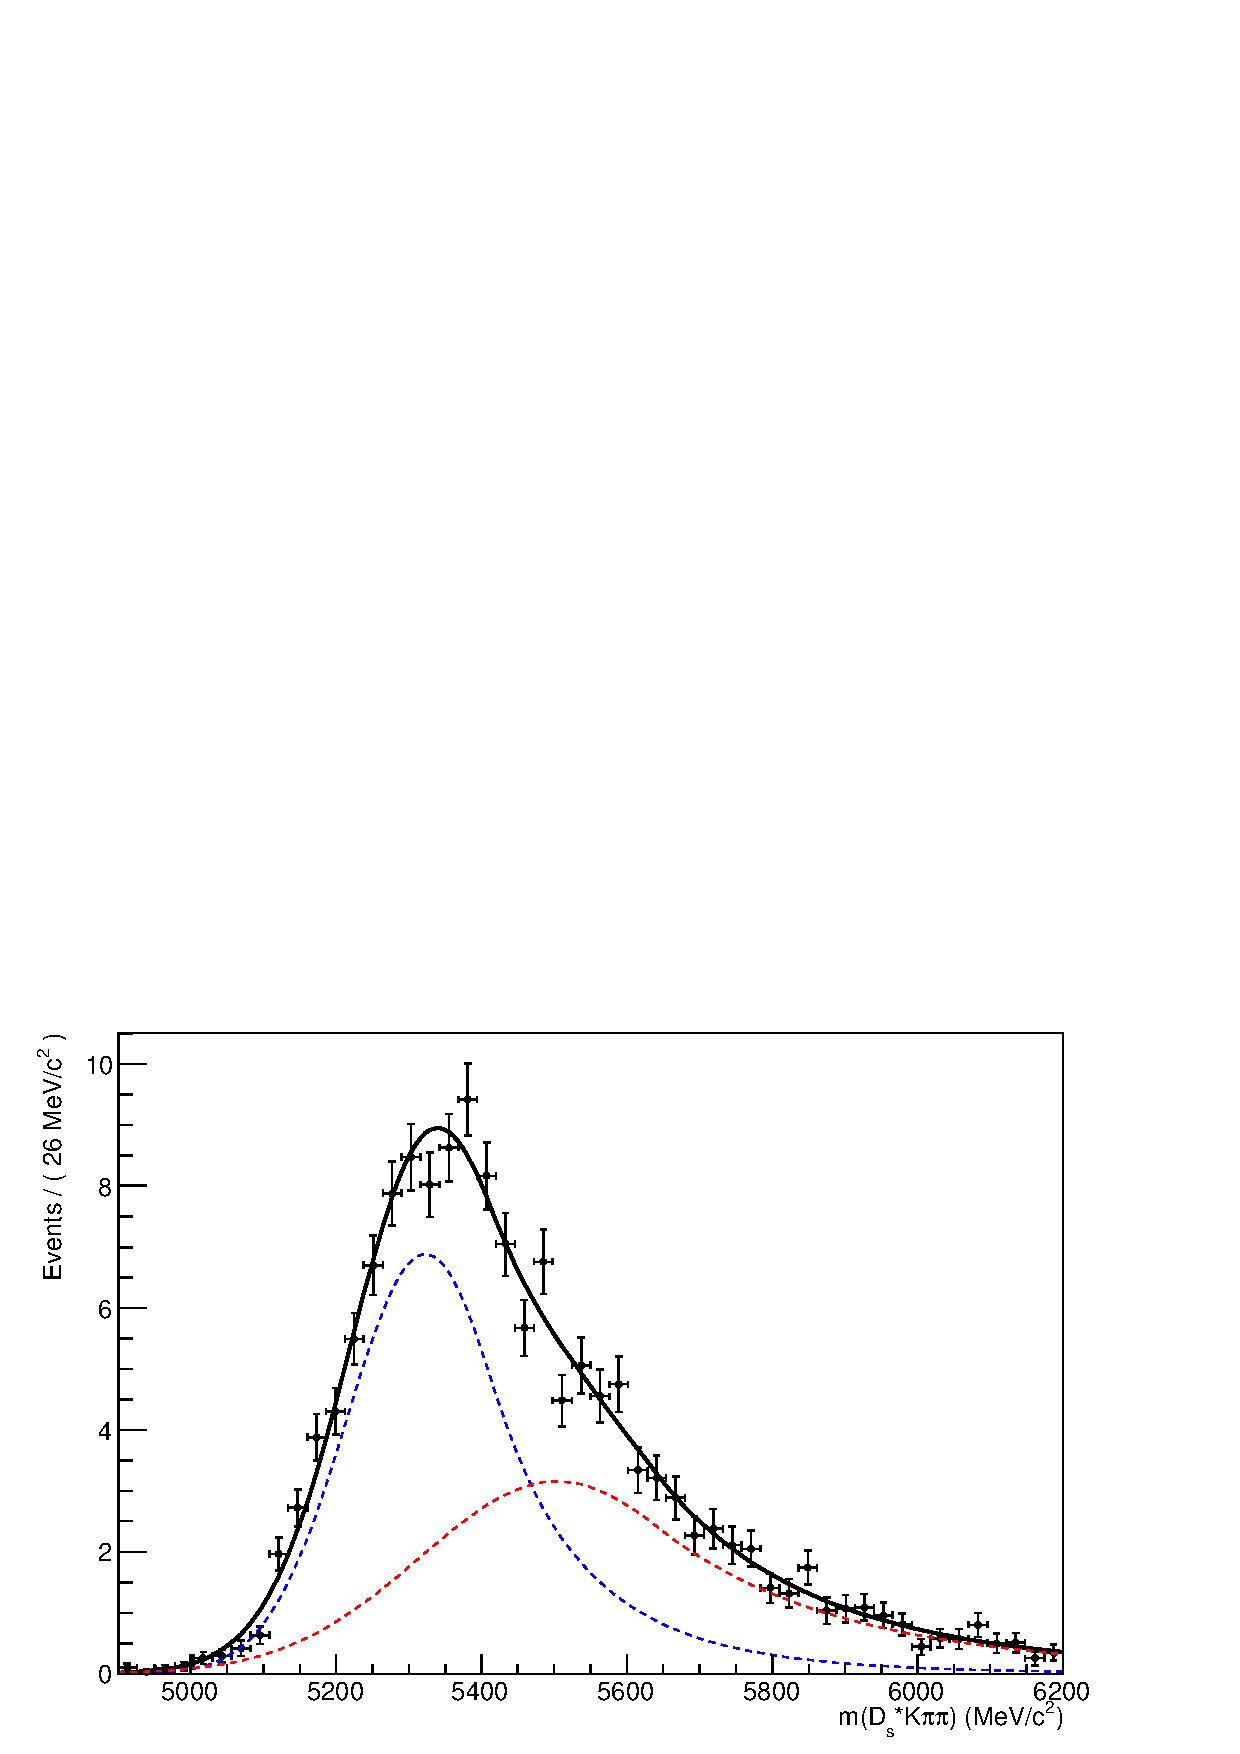
\includegraphics[width=4.5cm,height=2.0cm]{pics/Bs2Dsstarpipipi_as_DsKpipi.png}}\\
\subfigure{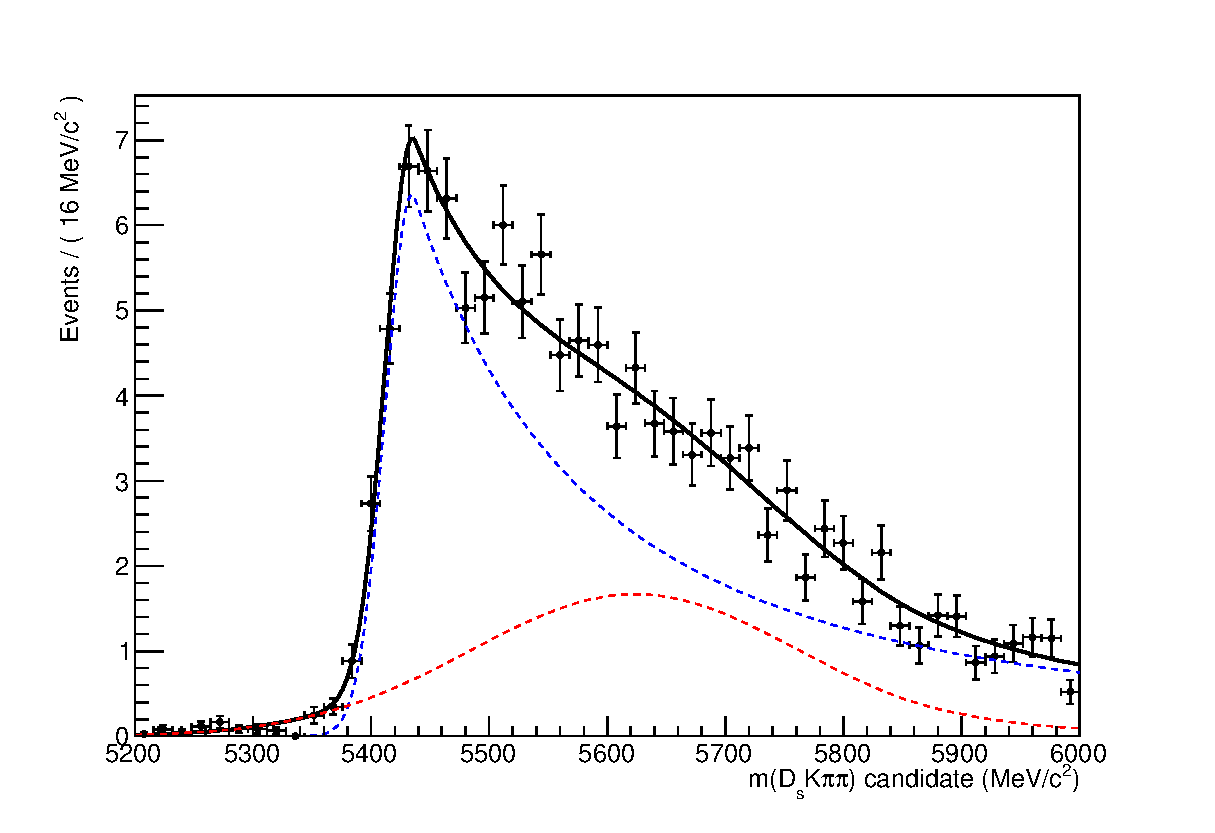
\includegraphics[width=4.5cm,height=2.0cm]{pics/Bs2Dspipipi_as_DsKpipi}}
\caption{top left: partially reconstructed $B_{s}\rightarrow D_{s}^{*}K\pi\pi$,\newline top right: $B_{s}\rightarrow D_{s}^{*}\pi\pi\pi$ miss-id, bottom: $B_{s}\rightarrow D_{s}\pi\pi\pi$ miss-id}
\end{figure}

\small

\textcolor{red}{Dangerous}: $B_{s}\rightarrow D_{s}^{(*)}\pi\pi\pi$ miss-id peaks in signal region $\rightarrow$ control contributions using PID calib
  
\normalsize

\end{frame}

\begin{frame}
\frametitle{Mass fits in normalization channel}

\begin{figure}
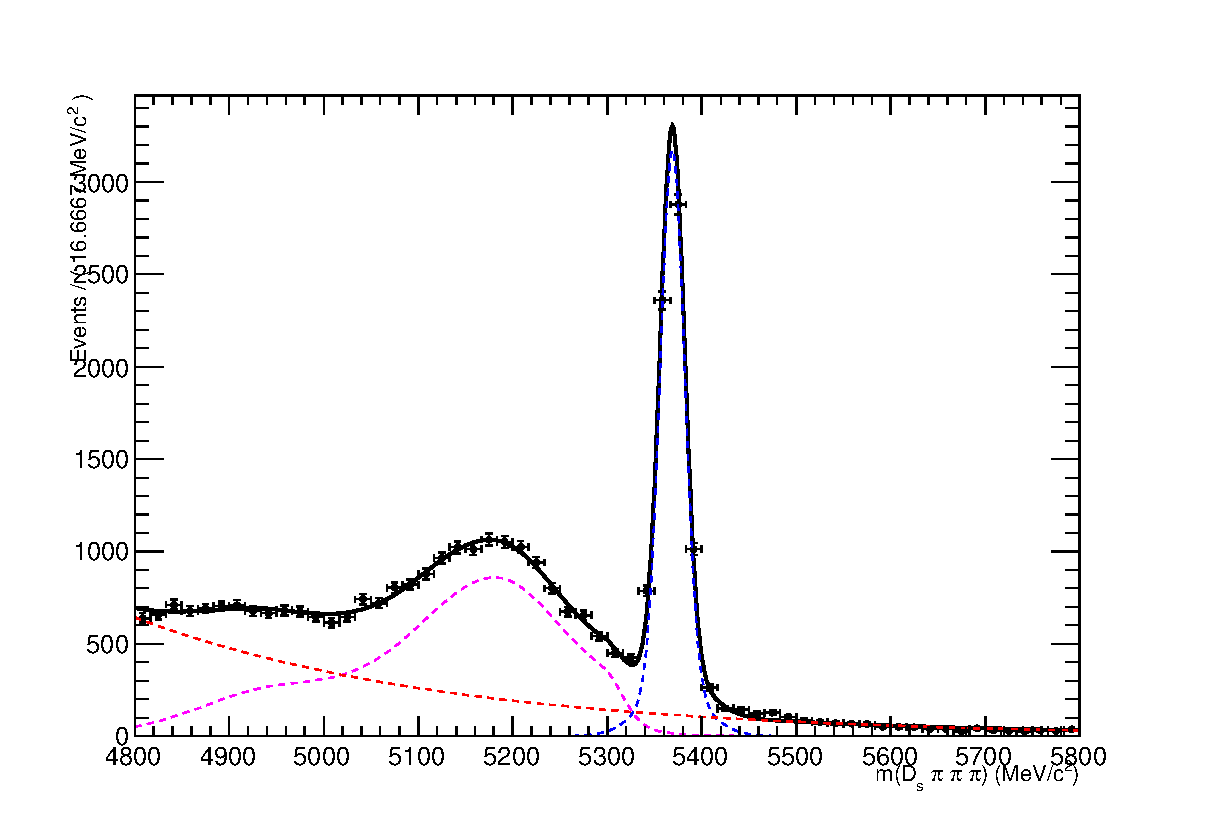
\includegraphics[width=5.4cm,height=3.8cm]{pics/3pi_BmassFit_11}
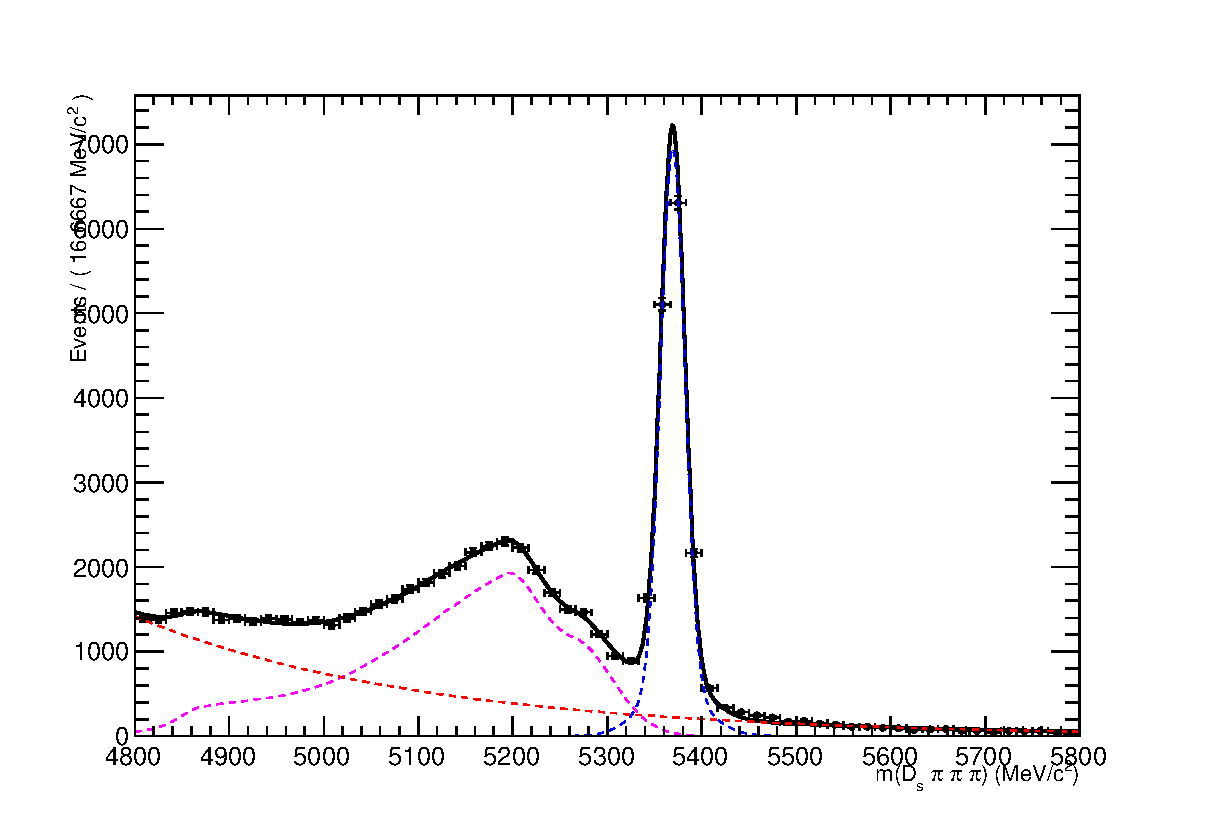
\includegraphics[width=5.4cm,height=3.8cm]{pics/3pi_BmassFit_12}\\
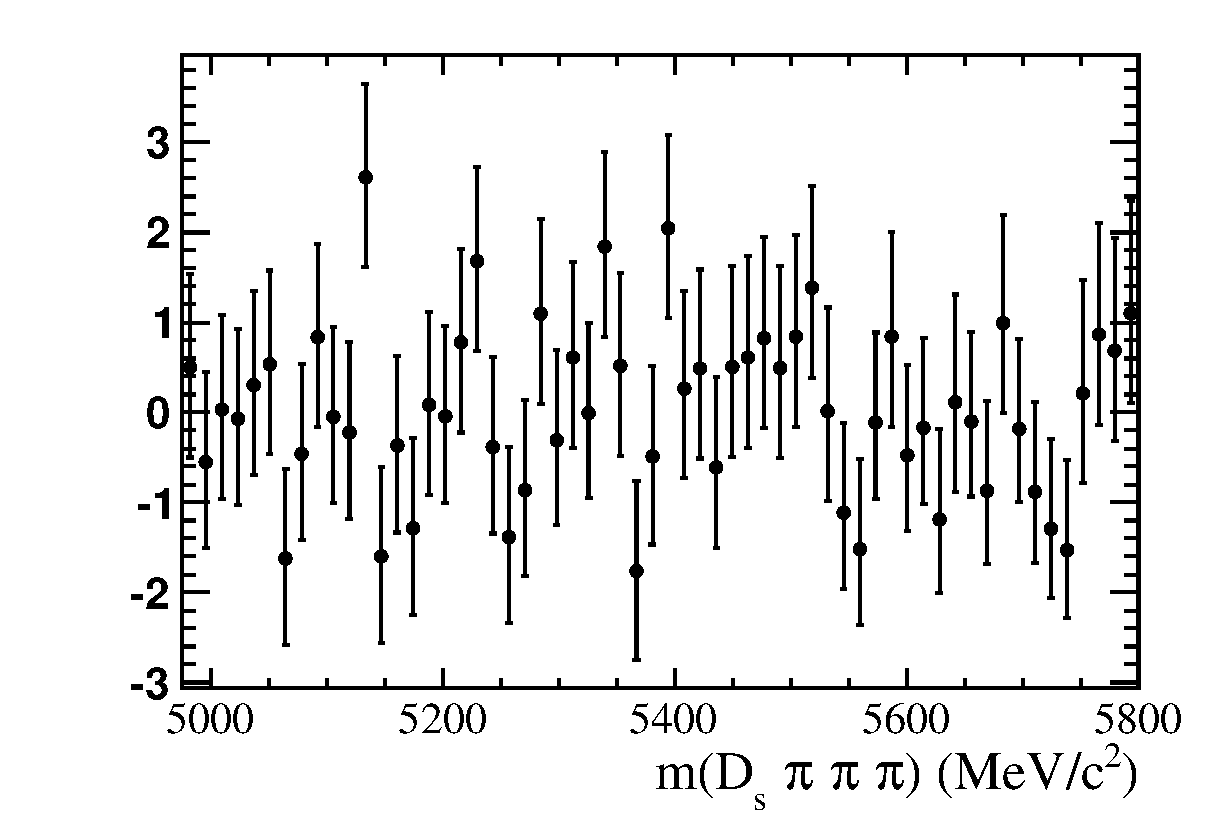
\includegraphics[width=5.4cm,height=1.5cm]{pics/3pi_pull_11}
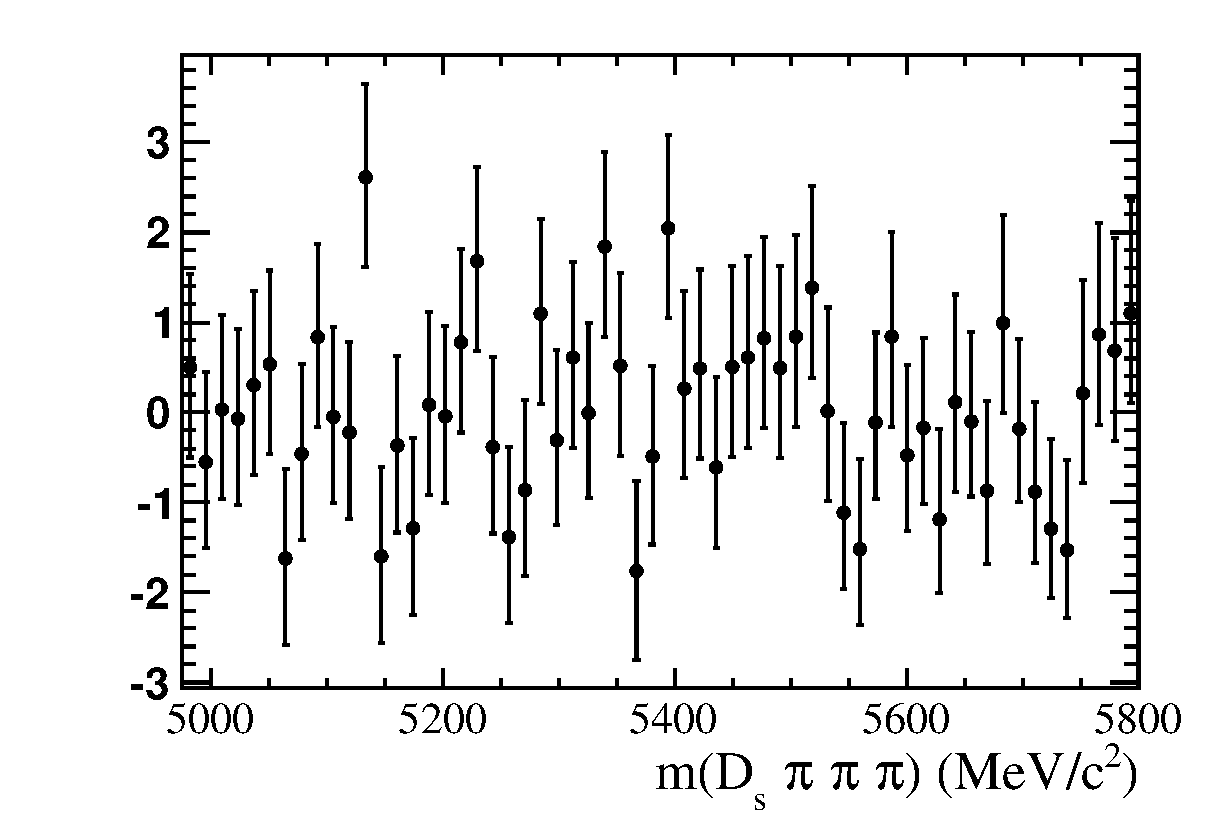
\includegraphics[width=5.4cm,height=1.5cm]{pics/3pi_pull_11}
\caption{Invariant mass distribution for $B_{s}\rightarrow D_{s}\pi\pi\pi$ candidates for (left) 2011 and (right) 2012}
\end{figure}

%$PDF(m_{B};\vec{\lambda}) = N_{Sig}\cdot DG(m_{B};\overline{m},\sigma) + N_{PhysBG}\cdot 3Bif.Gauss(m_{B};\overline{m},\sigma_{L},\sigma_{R}) + N_{comb}\cdot exp(m_{B};\alpha)$ \newline


\end{frame}

\begin{frame}
\frametitle{Mass fits in signal channel}

\begin{figure}
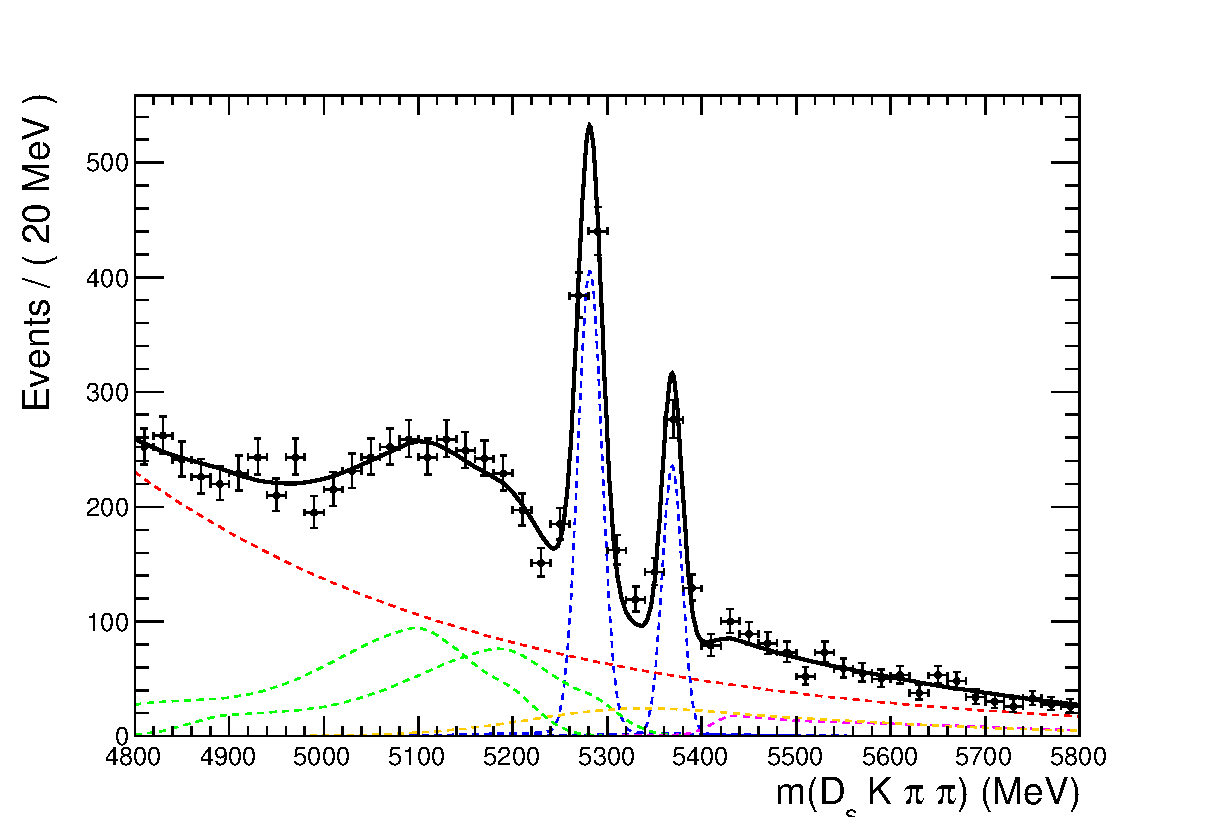
\includegraphics[width=5.4cm,height=3.8cm]{pics/BmassFit_11}
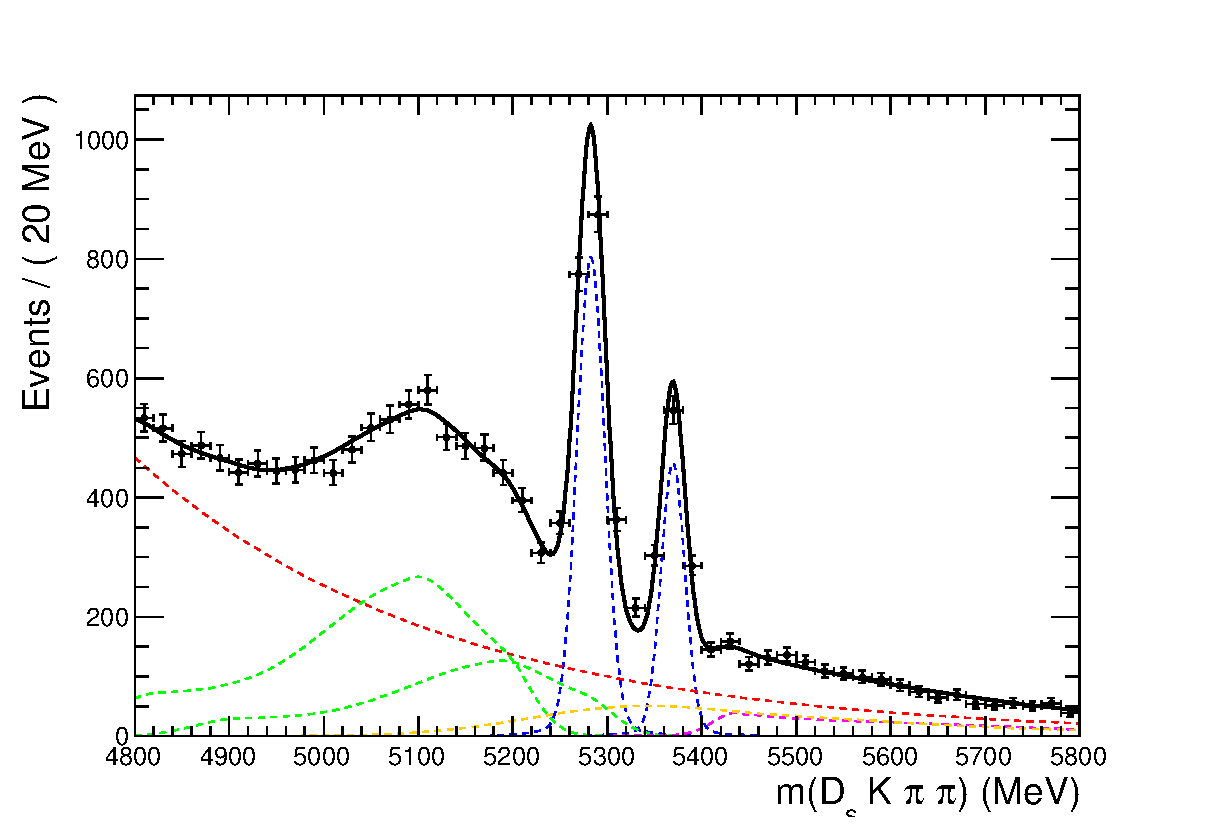
\includegraphics[width=5.4cm,height=3.8cm]{pics/BmassFit_12}\\
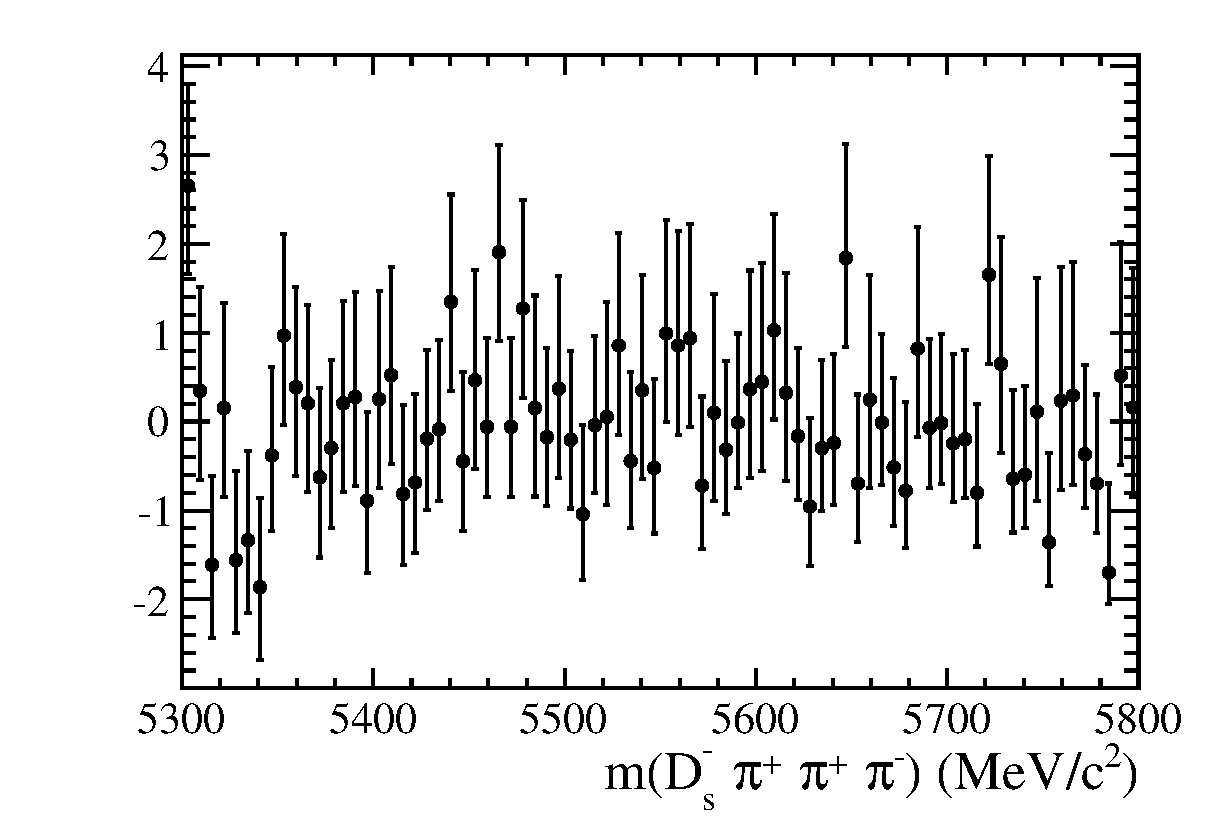
\includegraphics[width=5.4cm,height=1.5cm]{pics/pull_11}
\includegraphics[width=5.4cm,height=1.5cm]{pics/pull_12}
\caption{Invariant mass distribution for $B_{s}\rightarrow D_{s} K\pi\pi$ candidates for (left) 2011 and (right) 2012}
\end{figure}

%$PDF(m_{B};\vec{\lambda}) = N_{B^{0}}\cdot DG(m_{B^{0}};\overline{m},\sigma) + N_{Sig}\cdot DG(m_{B_{s}};\overline{m},\sigma) + N_{PhysBG}\cdot (3Bif.Gauss(m_{B};\overline{m},\sigma_{L},\sigma_{R}) + 2DCB(miss-id)) + N_{comb}\cdot exp(m_{B};\alpha)$ \newline

\end{frame}

\begin{frame}
\frametitle{Yields (not final, only $D_{s}\rightarrow K K \pi$)}

for the normalization channel we extract:

\begin{itemize}

\item 2011: $N_{B_{s}\rightarrow D_{s}\pi\pi\pi} = 4927 \pm 85$ \newline
\item 2012: $N_{B_{s}\rightarrow D_{s}\pi\pi\pi} = 14566 \pm 141$ \newline

\end{itemize}


and for the signal channel:

\begin{itemize}

\item 2011: $N_{B_{s}\rightarrow D_{s}K\pi\pi} = 201 \pm 21$ \newline
\item 2012: $N_{B_{s}\rightarrow D_{s}K\pi\pi} = 474 \pm 32$ \newline

\end{itemize}

\end{frame}



\begin{frame}
\frametitle{MC-Data comparison 1}

using the shown massfit we can get signal sWeights for data \newline

$\rightarrow$ compare distributions of sWeighted data and signal MC

\begin{figure}
\includegraphics[width=5.5cm,height=4.0cm]{pics/m_Kpipi_comp.png}
\subfigure{\includegraphics[width=5.5cm,height=4.0cm]{pics/m_pipi_comp.png}}
\end{figure}

\end{frame}

\begin{frame}
\frametitle{MC-Data comparison 2}

\begin{figure}
\includegraphics[width=5.5cm,height=4.0cm]{pics/p_KPlus_comp.png}
\subfigure{\includegraphics[width=5.5cm,height=4.0cm]{pics/p_piMinus_comp.png}}
\end{figure}

\end{frame}

\begin{frame}
\frametitle{MC-Data comparison 3}

\begin{figure}
\includegraphics[width=5.5cm,height=4.0cm]{pics/p_piPlus_comp.png}
\end{figure}

\end{frame}

\begin{frame}
\frametitle{MC-Data comparison 4}

\begin{figure}
\includegraphics[width=5.5cm,height=4.0cm]{pics/pt_Xs_comp.png}
\subfigure{\includegraphics[width=5.5cm,height=4.0cm]{pics/pt_Ds_comp.png}}
\end{figure}

\end{frame}

\begin{frame}
\frametitle{MC-Data comparison 5}

\begin{figure}
\includegraphics[width=5.5cm,height=4.0cm]{pics/max_ghostProb_comp.png}
\subfigure{\includegraphics[width=5.5cm,height=4.0cm]{pics/nTracks_comp.png}}
\end{figure}

\end{frame}

\begin{frame}
\frametitle{Outlook}

Next steps:

\begin{itemize}

\item check efficiencies between normalization and signal channel

\item make sure the PIDCalib samples are correct (some problems were reported): results crucial to fix yields of physical background which affects signal yield directly 

\item finalize the BR measurement: could be finished very quick, but depends strongly on my/our hardware occupancy (atm $99\%$ since November Testbeam) 

\item write ANA Note
			
\item move on to amplitude analysis 

%\item add $D_{s}\rightarrow \pi\pi\pi$ and $D_{s}\rightarrow K \pi \pi$ final states (began to look into this). Remember: \newline
	%		$BR(D_{s}\rightarrow K\pi\pi) \approx \frac{1}{10} \cdot BR(D_{s}\rightarrow KK\pi)$ \newline
	%		$BR(D_{s}\rightarrow \pi\pi\pi) \approx \frac{1}{5} \cdot BR(D_{s}\rightarrow KK\pi)$

\end{itemize}

\end{frame}

\appendix 
\addtocounter{framenumber}{-1} 

\begin{frame}
\thispagestyle{empty}
\bfseries\Huge

\begin{center}
BACKUP
\end{center}

\normalfont

\end{frame}

\begin{frame}
\frametitle{BDT Input 1}

\begin{figure}
\includegraphics[width=10.0cm,height=5.5cm]{pics/BDT_Input_12_1}
\end{figure}

\end{frame}
\begin{frame}
\frametitle{BDT Input 2}

\begin{figure}
\includegraphics[width=10.0cm,height=5.5cm]{pics/BD_Input_12_2}
\end{figure}

\end{frame}

\begin{frame}
\frametitle{BDT Input 3}

\begin{figure}
\includegraphics[width=10.0cm,height=5.5cm]{pics/BDT_Input_12_3}
\end{figure}

\end{frame}

\begin{frame}
\frametitle{BDT Input 4}

\begin{figure}
\includegraphics[width=10.0cm,height=5.5cm]{pics/BD_Input_12_4}
\end{figure}

\end{frame}

\begin{frame}
\frametitle{BDT Input correlation Signal}

\begin{figure}
\includegraphics[width=10.0cm,height=7.5cm]{pics/BDT_correlation_signal}
\end{figure}

\end{frame}


\begin{frame}
\frametitle{BDT Input correlation Background}

\begin{figure}
\includegraphics[width=10.0cm,height=7.5cm]{pics/BDT_correlation_background}
\end{figure}

\end{frame}

\begin{frame}
\frametitle{Time-dependent $\gamma$ determination}

%The decay rate for $B_{s}\to D_{s}^{-}K^{+}\pi^{+}\pi^{-} \equiv B_{s}\to f$ is:

\begin{equation*}
\begin{split}
\frac{d\Gamma_{B_{s}\to f}(t)}{dt} = \frac{1}{2}(1+|\lambda_{f}|^{2})e^{-\Gamma_{s}t} & [\cosh(\frac{\Delta\Gamma_{s}t}{2}) - \textcolor{green}{D_{f}}\sinh(\frac{\Delta\Gamma_{s}t}{2}) \\
& + \textcolor{red}{C_{f}}\cos(\Delta m_{s}t) - \textcolor{blue}{S_{f}}\sin(\Delta m_{s}t),]
\end{split}
\end{equation*}

with coefficients:

\begin{eqnarray*}
&\textcolor{green}{D_{f}} = \frac{2r_{D_{s}K\pi\pi}\cos(\Delta-(\gamma-2\beta_{s}))}{1 + r_{D_{s}K\pi\pi}^{2}}, 
\textcolor{red}{C_{f}} = \frac{1 - r_{D_{s}K\pi\pi}^{2}}{1 + r_{D_{s}K\pi\pi}^{2}}, \\
&\textcolor{blue}{S_{f}} = \frac{2r_{D_{s}K\pi\pi}\sin(\Delta-(\gamma-2\beta_{s}))}{1 + r_{D_{s}K\pi\pi}^{2}},
\end{eqnarray*}

with: \newline
$r_{D_{s}K\pi\pi} = \frac{A(\overline{B_{s}}\to D_{s}^{-}K^{+}\pi^{-}\pi^{+})}{A(B_{s}\to D_{s}^{-}K^{+}\pi^{-}\pi^{+})} = $ ratio of decay amplitudes and \\
$\Delta = $ strong phase difference \newline
\bfseries both vary over phase space \normalfont

\end{frame}


\end{document}